\section{Math 10 Derivatives Test}\label{math-10-derivatives-test}

\begin{enumerate}
\def\labelenumi{\arabic{enumi}.}
\tightlist
\item
  Let \(f(x)=\sqrt{x}\). What is the equation of the tangent line to
  \(f\) at the point \((4,2)\)?
\end{enumerate}

\begin{enumerate}
\def\labelenumi{(\Alph{enumi})}
\item
  \(y=\frac{1}{4} x+1\)
\item
  \(y=-\frac{1}{2} x+3\)
\item
  \(y=\frac{1}{2} x\)
\item
  \(y=2 x-6\)
\end{enumerate}

\begin{enumerate}
\def\labelenumi{\arabic{enumi}.}
\tightlist
\item
  What is the derivative of \(s(t)=\cos \left(t^2 + 1\right)\) ?
\end{enumerate}

\begin{enumerate}
\def\labelenumi{(\Alph{enumi})}
\item
  \(-2t\sin(t^2+1)\)
\item
  \(-(t^2+1)\sin(t^2+1)\)
\item
  \(\cos(2t)\)
\item
  \(-\sin(2t)\)
\end{enumerate}

\begin{enumerate}
\def\labelenumi{\arabic{enumi}.}
\setcounter{enumi}{2}
\tightlist
\item
  If \(f, g\), and \(h\) are nonzero differentiable functions, then the
  derivative of \(\frac{f}{h}\) is
\end{enumerate}

\begin{enumerate}
\def\labelenumi{(\Alph{enumi})}
\item
  \(\frac{f^{\prime} h - f h^{\prime}}{h^2}\)
\item
  \(\frac{f^{\prime} h + f h^{\prime}}{h^2}\)
\item
  \(\frac{f h^{\prime} - f^{\prime} h}{h^{2}}\)
\item
  \(\frac{f^{\prime}}{h^{\prime}}\)
\end{enumerate}

\begin{enumerate}
\def\labelenumi{\arabic{enumi}.}
\tightlist
\item
  The line tangent to the curve \(y=\sqrt{16-x}\) at the point \((0,4)\)
  has slope
\end{enumerate}

\begin{enumerate}
\def\labelenumi{(\Alph{enumi})}
\item
  8
\item
  4
\item
  \(1 / 8\)
\item
  \(-1 / 8\)
\item
  -8
\end{enumerate}

\begin{enumerate}
\def\labelenumi{\arabic{enumi}.}
\tightlist
\item
  If \(y=6 \ln (3 x)\) then what is \(y^{\prime}\) ?
\end{enumerate}

\begin{enumerate}
\def\labelenumi{(\Alph{enumi})}
\item
  \(\dfrac{6}{x}\)
\item
  \(\dfrac{2}{x}\)
\item
  \(\dfrac{1}{3x}\)
\item
  \(\dfrac{18}{x}\)
\end{enumerate}

\begin{enumerate}
\def\labelenumi{\arabic{enumi}.}
\tightlist
\item
  What is the value of
\end{enumerate}

\[
\lim _{\Delta x \rightarrow 0} \frac{2(x+\Delta x)^{2}-2 x^{2}}{\Delta x}
\]

\begin{enumerate}
\def\labelenumi{(\Alph{enumi})}
\item
  \(2 x\)
\item
  \(4 x\)
\item
  4
\item
  2
\item
  Does not exist
\end{enumerate}

\begin{enumerate}
\def\labelenumi{\arabic{enumi}.}
\setcounter{enumi}{7}
\tightlist
\item
  If \(w(t)=\sqrt{t^{2}-1}\) what is the value of \(w^{\prime}(4)\) ?
\end{enumerate}

\begin{enumerate}
\def\labelenumi{(\Alph{enumi})}
\item
  \(\frac{4}{\sqrt{15}}\)
\item
  \(\frac{2}{\sqrt{15}}\)
\item
  \(\frac{1}{\sqrt{15}}\)
\item
  \(\frac{1}{2 \sqrt{15}}\)
\end{enumerate}

\begin{enumerate}
\def\labelenumi{\arabic{enumi}.}
\setcounter{enumi}{8}
\tightlist
\item
  At which \(x\) value does the graph of \(y=3 x^{2}-10 x+15\) have a
  horizontal tangent line?
\end{enumerate}

\begin{enumerate}
\def\labelenumi{(\Alph{enumi})}
\item
  \(\frac{3}{5}\)
\item
  \(\frac{-3}{5}\)
\item
  \(\frac{5}{3}\)
\item
  \(\frac{-5}{3}\)
\end{enumerate}

\begin{enumerate}
\def\labelenumi{\arabic{enumi}.}
\tightlist
\item
  If \(h(x)=f\left(x^{2}+1\right)\) then which of the following is true?
\end{enumerate}

\begin{enumerate}
\def\labelenumi{(\Alph{enumi})}
\item
  \(h^{\prime}(x)=f^{\prime}\left(x^{2}+1\right)\)
\item
  \(h^{\prime}(x)=f^{\prime}(2 x)\)
\item
  \(h^{\prime}(x)=2 x f^{\prime}(2 x)\)
\item
  \(h^{\prime}(x)=2 x f^{\prime}\left(x^{2}+1\right)\)
\end{enumerate}

\begin{enumerate}
\def\labelenumi{\arabic{enumi}.}
\tightlist
\item
  If \(f(x)=\sin \left(2x +1\right)\) and \(g(x) = f^{\prime}(x)\), find
  \(g^{\prime}(x)\)
\end{enumerate}

\begin{enumerate}
\def\labelenumi{(\Alph{enumi})}
\item
  \(g^{\prime}(x) = -4 \sin (2x + 1)\)
\item
  \(g^{\prime}(x) = 2 \sin (2x + 1)\)
\item
  \(g^{\prime}(x) = 4 \sin(2x + 1) \cos(2x + 1)\)
\item
  \(g^{\prime}(x) = -4x \cos(2x + 1)\)
\end{enumerate}

\begin{enumerate}
\def\labelenumi{\arabic{enumi}.}
\tightlist
\item
  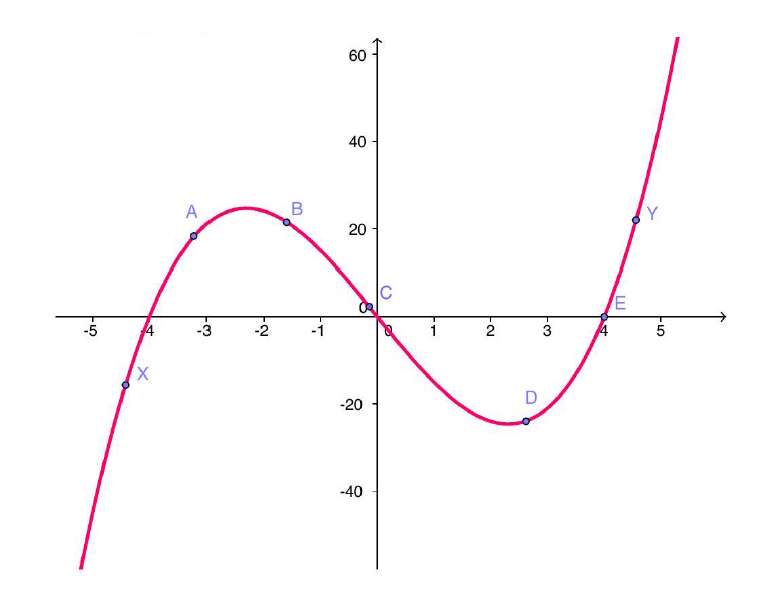
\includegraphics{graph1.PNG} Given the graph of \(f(x)\) below, select
  which statement is true about values of \(f'(x)\)
\end{enumerate}

\begin{enumerate}
\def\labelenumi{(\Alph{enumi})}
\tightlist
\item
  \(f'(C) < f'(D) < f'(Y)\)
\item
  \(f'(A) < f'(B) < f'(C)\)
\item
  \(f'(X) < f'(Y) < f'(C)\)
\item
  \(f'(X) < f'(B) < f'(E)\)
\end{enumerate}

\begin{enumerate}
\def\labelenumi{\arabic{enumi}.}
\tightlist
\item
  Let \(f(x)=x^{3}-6 x^{2}+10\). At which point(s) on the graph of \(f\)
  is the tangent line parallel to the line \(15 x-y=11\) ?
\end{enumerate}

\begin{enumerate}
\def\labelenumi{(\Alph{enumi})}
\item
  \((2,-6)\) and \((-2,22)\)
\item
  \((2,-6)\) and \((-2,-22)\)
\item
  \((5,-15)\) and \((-1,3)\)
\item
  \((5,-15)\) and \((2,-6)\)
\end{enumerate}

\begin{center}\rule{0.5\linewidth}{0.5pt}\end{center}

\begin{enumerate}
\def\labelenumi{\arabic{enumi}.}
\tightlist
\item
  If \(y(x) = \dfrac{sin(2x)}{x^2}\) find \(y'(x)\)
\end{enumerate}

\begin{enumerate}
\def\labelenumi{(\Alph{enumi})}
\tightlist
\item
  \(\dfrac{(2 x cos(2 x) - 2 sin(2 x))}{x^3}\)
\item
  \(\dfrac{ 2 \cos(2x)}{x}\)
\item
  \(\dfrac{ x^2 \cos(2x) - 1 \sin(2x)} { x^3}\)
\item
  \(\dfrac{ x^2 sin(2x) + 2 \cos(2x)} {x^4}\)
\end{enumerate}

\begin{enumerate}
\def\labelenumi{\arabic{enumi}.}
\setcounter{enumi}{1}
\tightlist
\item
  Calculate \(\dfrac{d}{dt} \left( \ln(e^{2t}) - t^2 \right)\)
\end{enumerate}

\begin{enumerate}
\def\labelenumi{(\Alph{enumi})}
\tightlist
\item
  2
\item
  \(\dfrac{1}{2t}\)
\item
  \(\dfrac{2}{e^{2t}}\)
\item
  \(\dfrac{1}{2e^{2t}}\)
\end{enumerate}

That's taht

\begin{longtable}[]{@{}
  >{\raggedright\arraybackslash}p{(\columnwidth - 10\tabcolsep) * \real{0.1200}}
  >{\raggedright\arraybackslash}p{(\columnwidth - 10\tabcolsep) * \real{0.2000}}
  >{\raggedright\arraybackslash}p{(\columnwidth - 10\tabcolsep) * \real{0.2000}}
  >{\raggedright\arraybackslash}p{(\columnwidth - 10\tabcolsep) * \real{0.2133}}
  >{\raggedright\arraybackslash}p{(\columnwidth - 10\tabcolsep) * \real{0.0533}}
  >{\raggedright\arraybackslash}p{(\columnwidth - 10\tabcolsep) * \real{0.2133}}@{}}
\toprule\noalign{}
\begin{minipage}[b]{\linewidth}\raggedright
x
\end{minipage} & \begin{minipage}[b]{\linewidth}\raggedright
0
\end{minipage} & \begin{minipage}[b]{\linewidth}\raggedright
1
\end{minipage} & \begin{minipage}[b]{\linewidth}\raggedright
2
\end{minipage} & \begin{minipage}[b]{\linewidth}\raggedright
3
\end{minipage} & \begin{minipage}[b]{\linewidth}\raggedright
4
\end{minipage} \\
\midrule\noalign{}
\endhead
\bottomrule\noalign{}
\endlastfoot
\(f(x)\) & \(\frac{1}{2}\) & \(\frac{1}{3}\) & 1 & -1 & 3 \\
\(g(x)\) & -2 & 1 & \(-\frac{1}{2}\) & 2 & \(-\frac{1}{3}\) \\
\(f'(x)\) & \(\frac{3}{2}\) & \(\frac{5}{3}\) & \(\frac{1}{4}\) & 0 &
\(-frac{4}{5}\) \\
\(g'(x)\) & \(-1\) & \(\frac{2}{3}\) & -4 & -3 & \(-\frac{1}{3}\) \\
\end{longtable}

Calculate the following

\begin{enumerate}
\def\labelenumi{(\Alph{enumi})}
\tightlist
\item
  1
\item
  2
\end{enumerate}

\begin{center}\rule{0.5\linewidth}{0.5pt}\end{center}

\subsection{5. AP Calculus AB: Section
II}\label{ap-calculus-ab-section-ii}

Instructions: In the questions below, find the indicated derivatives
using the following definitions

\[
\begin{aligned}
p(x) & =f(x) g(x) \\
q(x) & =\frac{f(x)}{g(x)} \\
c(x) & =f(g(x)) \\
s(x) & =f(2 x)
\end{aligned}
\]

\begin{enumerate}
\def\labelenumi{\arabic{enumi}.}
\tightlist
\item
  \(f^{\prime}(4)=\)
\item
  \(g^{\prime}(-1)=\)
\item
  \(p^{\prime}(1)=\)
\item
  \(q^{\prime}(1)=\)
\item
  \(c^{\prime}(-1)=\)
\item
  \(s^{\prime}(3)=\)
\item
  \(p^{\prime}(7)=\)
\end{enumerate}
